%%%%%%%%%%%%%%%%%%%%%%%%%%%%%%%%%%%%%%%%%
%
% CMPT 435
% Fall 2022
% Assignment 4
%
%%%%%%%%%%%%%%%%%%%%%%%%%%%%%%%%%%%%%%%%%

%%%%%%%%%%%%%%%%%%%%%%%%%%%%%%%%%%%%%%%%%
% Short Sectioned Assignment
% LaTeX Template
% Version 1.0 (5/5/12)
%
% This template has been downloaded from: http://www.LaTeXTemplates.com
% Original author: % Frits Wenneker (http://www.howtotex.com)
% License: CC BY-NC-SA 3.0 (http://creativecommons.org/licenses/by-nc-sa/3.0/)
% Modified by Alan G. Labouseur  - alan@labouseur.com
%
%%%%%%%%%%%%%%%%%%%%%%%%%%%%%%%%%%%%%%%%%

%----------------------------------------------------------------------------------------
%	PACKAGES AND OTHER DOCUMENT CONFIGURATIONS
%----------------------------------------------------------------------------------------

\documentclass[letterpaper, 10pt,DIV=13]{scrartcl} 

\usepackage[T1]{fontenc} % Use 8-bit encoding that has 256 glyphs
\usepackage[english]{babel} % English language/hyphenation
\usepackage{amsmath,amsfonts,amsthm,xfrac} % Math packages
\usepackage{sectsty} % Allows customizing section commands
\usepackage{graphicx}
\usepackage{algorithm, algpseudocode}
\usepackage{listings}
\usepackage{parskip}
\usepackage{lastpage}
\usepackage{color}
\usepackage{qtree}
\usepackage{tikz}

\allsectionsfont{\normalfont\scshape} % Make all section titles in default font and small caps.

\usepackage{fancyhdr} % Custom headers and footers
\pagestyle{fancyplain} % Makes all pages in the document conform to the custom headers and footers

\fancyhead{} % No page header - if you want one, create it in the same way as the footers below
\fancyfoot[L]{} % Empty left footer
\fancyfoot[C]{} % Empty center footer
\fancyfoot[R]{page \thepage\ of \pageref{LastPage}} % Page numbering for right footer

\renewcommand{\headrulewidth}{0pt} % Remove header underlines
\renewcommand{\footrulewidth}{0pt} % Remove footer underlines
\setlength{\headheight}{13.6pt} % Customize the height of the header

\numberwithin{equation}{section} % Number equations within sections (i.e. 1.1, 1.2, 2.1, 2.2 instead of 1, 2, 3, 4)
\numberwithin{figure}{section} % Number figures within sections (i.e. 1.1, 1.2, 2.1, 2.2 instead of 1, 2, 3, 4)
\numberwithin{table}{section} % Number tables within sections (i.e. 1.1, 1.2, 2.1, 2.2 instead of 1, 2, 3, 4)

\setlength\parindent{0pt} % Removes all indentation from paragraphs.

\binoppenalty=3000
\relpenalty=3000

\algrenewcommand{\algorithmiccomment}[1]{\hskip1em\textit{$//$ #1}}

%----------------------------------------------------------------------------------------
%	TITLE SECTION
%----------------------------------------------------------------------------------------

\newcommand{\horrule}[1]{\rule{\linewidth}{#1}} % Create horizontal rule command with 1 argument of height

\title{	
   \normalfont \normalsize 
   \textsc{CMPT 435 - Fall 2022 - Dr. Labouseur} \\[10pt] % Header stuff.
   \horrule{0.5pt} \\[0.25cm] 	% Top horizontal rule
   \huge Assignment Four  \\     	    % Assignment title
   \horrule{0.5pt} \\[0.25cm] 	% Bottom horizontal rule
}

\author{Josh Seligman \\ \normalsize joshua.seligman1@marist.edu}

\date{\normalsize\today} 	% Today's date.

\begin{document}
\maketitle % Print the title

\section{Binary Search Tree}\label{bstSection}
\subsection{The Data Structure}
A binary search tree is a data structure that, for each node in the tree, all child nodes on its left are less than the value and all child nodes on the right are greater than or equal to the value in the given node. Therefore, when performing an in-order traversal by printing out all left-hand nodes, then the value of the given node, and lastly all of the right-hand nodes, all values will be printed out in order. As shown in Figures \ref{figure:bstNormal} and \ref{figure:bstBad}, the values are inserted into the tree in the order in which they are received. This can impact the time it takes to traverse the tree to find a given element, which will be examined in Section \ref{bstAnalysis}.

\hspace*{\fill}
\begin{figure}
  \caption{Sample binary search tree for the numbers 5, 3, 1, 2, 7, 6, 8.}
  \label{figure:bstNormal}
  % Documentation: https://www.ling.upenn.edu/advice/latex/qtree/qtreenotes.pdf
  \Tree [.5
          [.3
            [.1
              [.{null} ]
              [.2 ]
            ]
            [.{null} ]
          ]
          [.7
            [.6 ]
            [.8 ]
          ]
        ]
\end{figure}
\hspace*{\fill}

\hspace*{\fill}
\begin{figure}
  \caption{Sample binary search tree for the numbers 1, 2, 3, 5, 6, 7, 8.}
  \label{figure:bstBad}
  % Documentation: https://www.ling.upenn.edu/advice/latex/qtree/qtreenotes.pdf
  \Tree [.1
          [.{null} ]
          [.2 
            [.{null} ]
            [.3 
              [.{null} ]
              [.5 
                [.{null} ]
                [.6 
                  [.{null} ]
                  [.7 
                    [.{null} ]
                    [.8 ]
                  ]
                ]
              ]
            ]
          ]
        ]
\end{figure}
\hspace*{\fill}


\begin{algorithm}
  \caption{Binary Search Tree Lookup. Assume $cur$ starts off as the root of the tree.}
  \label{algorithm:bstLookup}
  %Documentation for algorithmicx: https://texdoc.org/serve/algorithmicx/0
  \begin{algorithmic}[1]
    \Procedure{BSTLookup}{$target$, $cur$}
      \State $out \gets false$ \Comment{Assume target is not found}
      \If{$target== cur.val$}
        \State $out \gets true$ \Comment{Found the target value}
      \ElsIf{$target < cur.val$}
        \State $out \gets BSTLookup(target, cur.left)$ \Comment{Target is on the left}
      \Else \Comment{$target \geq cur.val$}
        \State $out \gets BSTLookup(target, cur.right)$ \Comment{Target is on the right}
      \EndIf
      \State \Return $out$
    \EndProcedure
  \end{algorithmic}
\end{algorithm}

\subsection{Asymptotic Analysis}\label{bstAnalysis}
Algorithm \ref{algorithm:bstLookup} provides the pseudocode for performing a lookup on a binary search tree. As shown on lines 6 and 8, the area of the tree gets cut in half for each level of the recursion tree. This causes the expected runtime for a binary search tree lookup to be the same as binary search at $O(log_2n)$. However, as displayed in Figures \ref{figure:bstNormal} and \ref{figure:bstBad}, the order in which the data arrive makes a huge difference in the number of checks needed to find an element. For instance, when looking for the number 8 in the tree in Figure \ref{figure:bstNormal}, it will start with the 5 and go to the right because 8 > 5, then compare 8 with the 7 and also go to the right because 8 > 7, and then end when it finds the 8. Since there are 7 elements in the tree, it should take around $log_{2}7$ comparisons to find an element, and 3 comparisons is very close to the expected outcome. However, when trying to find 8 in the tree in Figure \ref{figure:bstBad}, one will have to compare 8 with every single element in the tree, which degrades the binary search tree lookup to be $O(n)$ as it is just doing a linear search. Therefore, when working with a binary search tree, it is important to make sure the data are shuffled in a random order to ensure the tree is as close to being balanced as possible. Since shuffling is an $O(n)$ operation, taking the time to shuffle a sorted array before putting the data in a binary search tree will save a lot of time in the long run especially when doing a lot of lookups within the tree.

\section{Graphs}
\subsection{The Data Structure}
A graph is a data structure that is composed of vertices that are connected via edges. Graphs can be useful for modeling networks of objects, such as LinkedIn connections or the many locations within a city map. The edges that connect the vertices together may have direction and weights, but this paper will focus on undirected and unweighted graphs. As illustrated in Figure \ref{figure:graph}, some of the vertices are connected to each other with various levels of cardinality. Additionally, some vertices may be disconnected from some areas of the graph. This is the case with vertices 6 and 7, which are on their own island separate from the rest of the graph.

\begin{figure}
  \hspace*{\fill}
  % From https://www.baeldung.com/cs/latex-drawing-graphs
  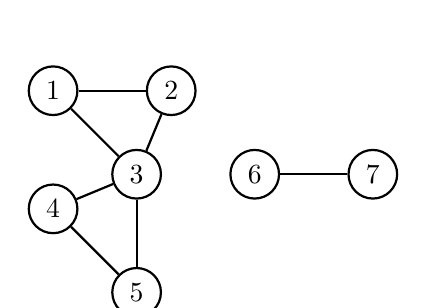
\begin{tikzpicture}[node distance={15mm}, thick, main/.style = {draw, circle}] 
    \node[main] (1) {$1$};
    \node[main] (2) [right of=1] {$2$};
    \node[main] (3) [below right of=1] {$3$};
    \node[main] (4) [below of=1] {$4$};
    \node[main] (5) [below right of=4] {$5$};
    \node[main] (6) [right of=3] {$6$};
    \node[main] (7) [right of=6] {$7$};
    \draw (1) -- (2);
    \draw (1) -- (3);
    \draw (2) -- (3);
    \draw (3) -- (4);
    \draw (5) -- (4);
    \draw (3) -- (5);
    \draw (6) -- (7);
  \end{tikzpicture}
  \hspace*{\fill}
  \caption{Sample undirected, unweighted graph consisting of 7 vertices and 7 edges.}
  \label{figure:graph}
\end{figure}

% Colors and lstset for syntax highlighting from https://www.overleaf.com/latex/examples/syntax-highlighting-in-latex-with-the-listings-package/jxnppmxxvsvk
\definecolor{mygreen}{rgb}{0,0.6,0}
\definecolor{mygray}{rgb}{0.5,0.5,0.5}
\definecolor{mymauve}{rgb}{0.58,0,0.82}
\lstset{
  backgroundcolor=\color{white},   % choose the background color
  basicstyle=\footnotesize,        % size of fonts used for the code
  breaklines=true,                 % automatic line breaking only at whitespace
  captionpos=b,                    % sets the caption-position to bottom
  commentstyle=\color{mygreen},    % comment style
  escapeinside={\%*}{*},          % if you want to add LaTeX within your code
  keywordstyle=\color{blue},       % keyword style
  stringstyle=\color{mymauve},     % string literal style
}

\subsection{Binary Search Tree}
\lstinputlisting[caption = Binary Search Tree Lookup (C++), label = lst:bstLookup, language = C++, firstline = 74, lastline = 107, firstnumber = 1]{./../binarySearchTree.cpp}

\subsection{Graphs}
\lstinputlisting[caption = Graph Depth First Search (C++), label = lst:graphDfs, language = C++, firstline = 213, lastline = 246, firstnumber = 1]{./../graph.cpp}

\lstinputlisting[caption = Graph Breadth First Search (C++), label = lst:graphBfs, language = C++, firstline = 248, lastline = 295, firstnumber = 1]{./../graph.cpp}

\end{document}